\subsubsection{Obstacle Avoidance Through Odometric Sensors}
Wireless communication between devices is always prospect to errors and obstructions, as such a way had to be devised so that the rover will function safely when communications fail whilst also avoiding a significant decline in the system's life expectancy.\\In order to achieve this, several odometric sensors will be placed on the rover, covering the \ang{360} radius, and whenever it judges an obstacle is too close (through the feedback of the sensors) it will not follow commands that would force it to get any closer to said obstacle.\\The implementation of an autonomous obstacle avoidance algorithm was considered, however implementing such an algorithm would, in the best scenario, remove control from the user and, in the worst scenario, enter into direct conflict with the latter. Therefore, since neither of the aforementioned scenarios was in the best interests of either the system or the user, it was opted to simply force the system to stop if a command would take it too close to an obstacle and to not allow it to move towards it any further.
\subsubsection{Obstacle Avoidance Simulations}
In order to plot the rover's path on a 2D diagram, the \textit{Mobile Robotics Simulation Toolbox}, made available by MATLAB, will be used. A series of waypoints  (these will simulate the user's commands) will be placed on a 2D map with borders, the latter of which will be used as obstacles. The waypoints shall direct the rover towards one of the borders in a turn and a straight line. Ideally the rover will stop before reaching the obstacle whilst also keeping enough space to turn away from it.\\
\\
The initial position of the rover shall be at coordinates (1,1) and an angle of 0 rads, as depicted in Fig.~\ref{fig:iniState}. 
From this standpoint, two simulations will be considered: a straight line that will require a $\frac{\pi}{2}$ rads turn upward (this turn serves to test the algorithm, to make sure it does not stop changes in direction whilst away from obstacles) and head straight towards one of the walls of the map;
and a second simulation, involving a turn towards a wall. In order either simulation to be a success the rover must stop before crashing against the wall with enough space to steer away from the obstacle.

\begin{figure}[!htbp]
\centering
       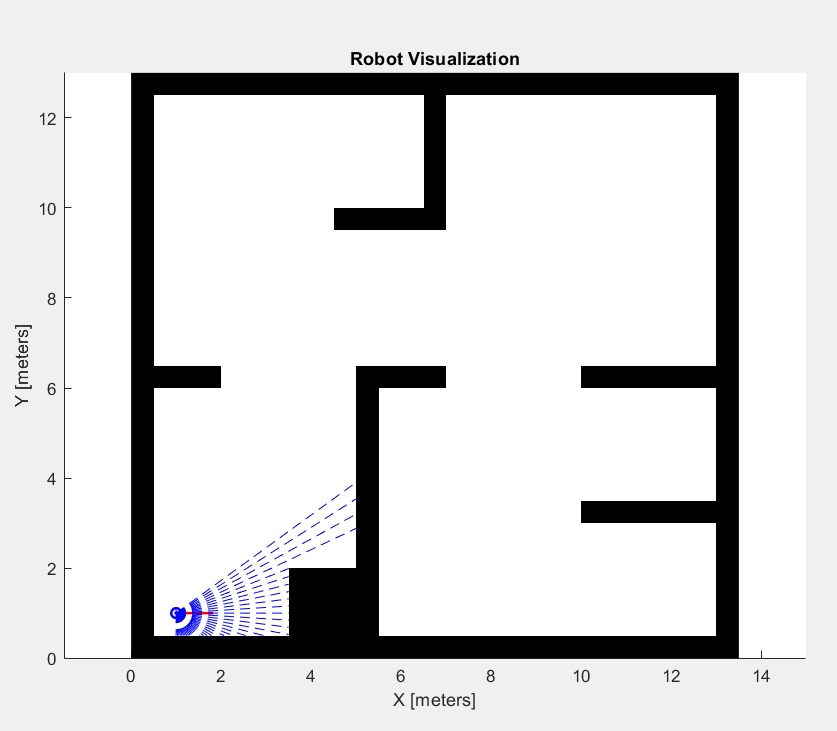
\includegraphics[page=1,width=0.55\textwidth]{img/startState.png} 
\caption{Initial State of simulation}
\label{fig:iniState}
\end{figure}

Firstly it must turn towards the wall, Fig~\ref{fig:sim1Turn}.
\begin{figure}[!htbp]
\centering
       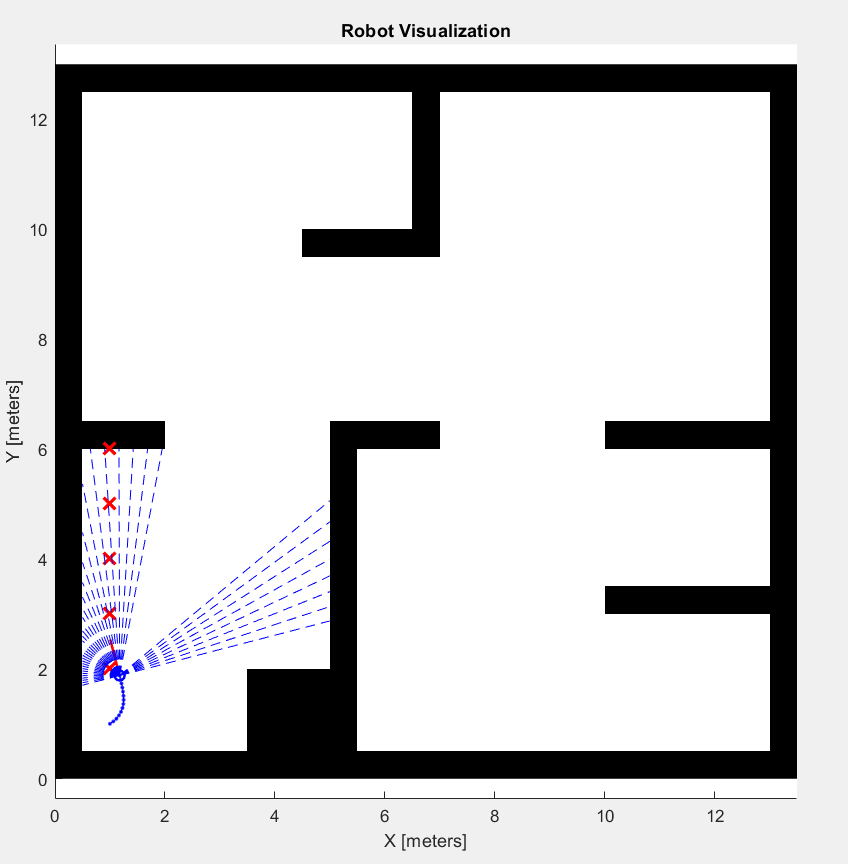
\includegraphics[page=1,width=0.55\textwidth]{img/line2.png} 
\caption{After Rover Turns Towards Wall}
\label{fig:sim1Turn}
\end{figure}

Afterwards it must head in a straight line and stop before the obstacle, Fig~\ref{fig:sim2Line}

\begin{figure}[!htbp]
\centering
       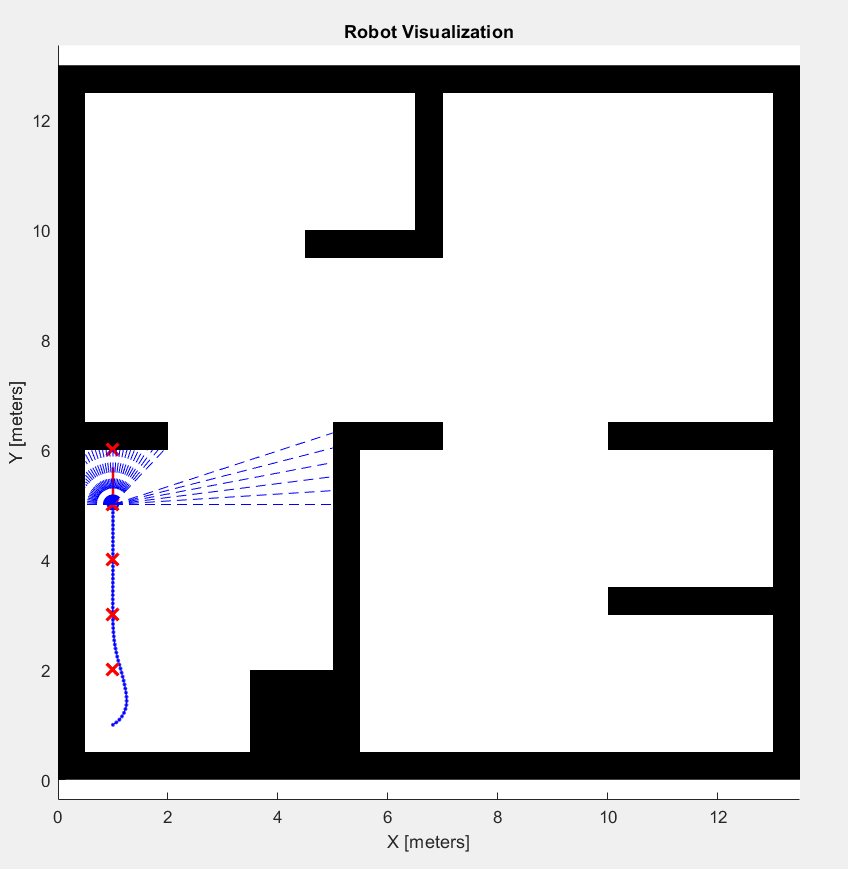
\includegraphics[page=1,width=0.55\textwidth]{img/line3.png} 
\caption{Rover Stopped Before Reaching Wall}
\label{fig:sim2Line}
\end{figure}

In the second simulation, which shall start, once again from the initial position depicted in Fig.~\ref{fig:iniState}, the rover must turn towards a path that avoids the right wall, Fig.~\ref{fig:sim2Line} and afterwards turn again and stop before reaching the wall with enough space to turn away from the latter, Fig.~\ref{fig:sim3Line}.

\begin{figure}[!htbp]
\centering
       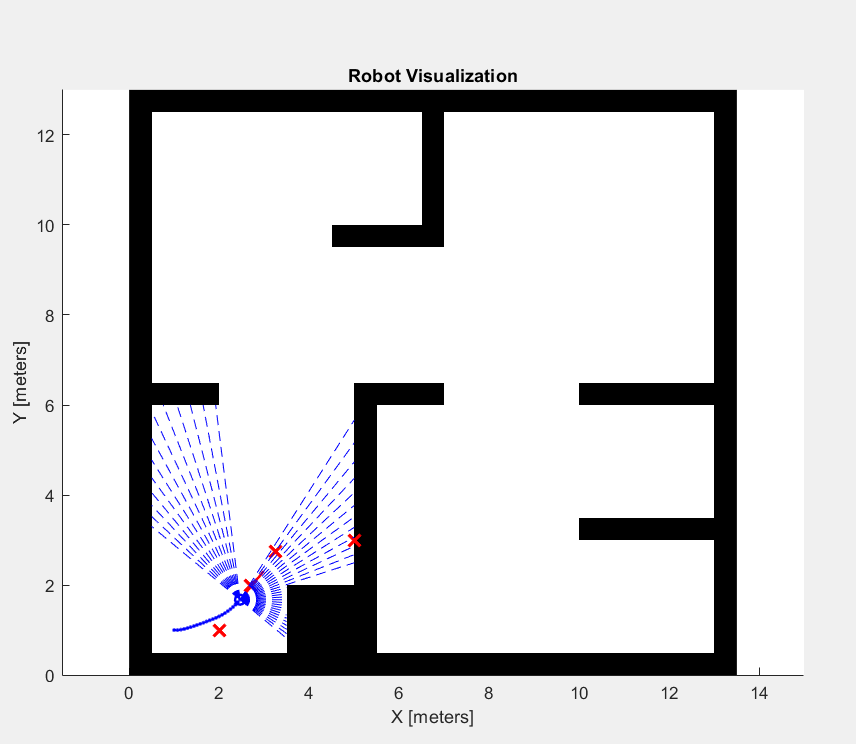
\includegraphics[page=1,width=0.6\textwidth]{img/turn2.png} 
\caption{Rover Starts the Turn}
\label{fig:sim2Line}
\end{figure}

\begin{figure}[!htbp]
\centering
       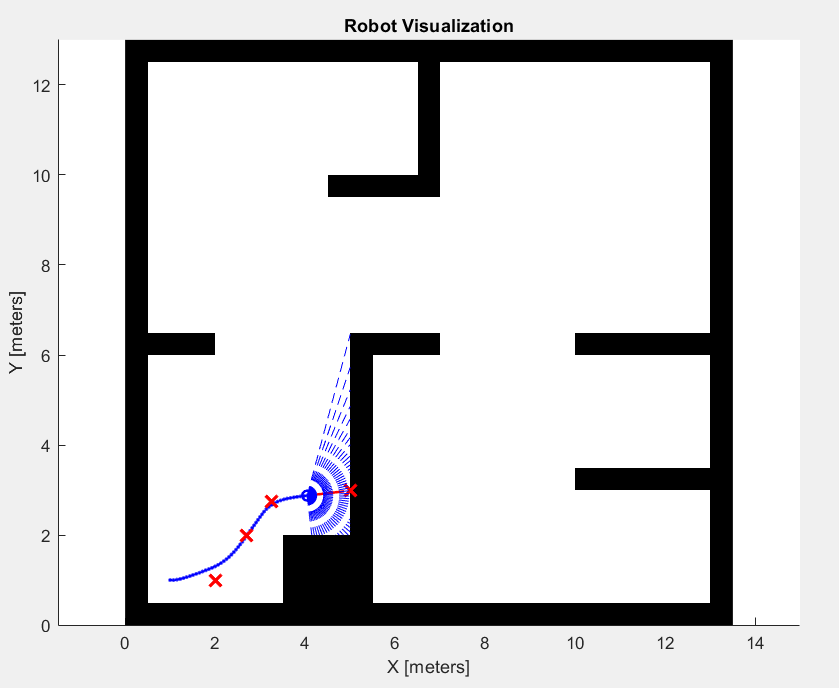
\includegraphics[page=1,width=0.6\textwidth]{img/turn3.png} 
\caption{Rover Turned and Stopped Before Reaching Wall}
\label{fig:sim3Line}
\end{figure}
\newpage

\subsubsection{Odometric Sensor} 
For the obstacle avoidance, several of \href{https://www.botnroll.com/pt/infravermelhos/158-sen-00242.html}{GP2Y0A21YK Infrared Sensors} (Fig~\ref{fig:sensor}) will be placed on the rover, since it has an allowable field angle of up to \ang{40}, this would mean at least 9 sensors would be required to cover \ang{360}, this is assuming that they are placed in such a way that there is no overlap, however since any sort of "blind spot" will place the rover in jeopardy, some overlap is desired. Considering the rover's dimensions, it is unlikely that 9 sensors can be placed upon it with enough overlap to completely cover the \ang{360}, therefore it is likely that a few more will have to placed to guarantee safety of the rover.

\begin{figure}[!htbp]
\centering
       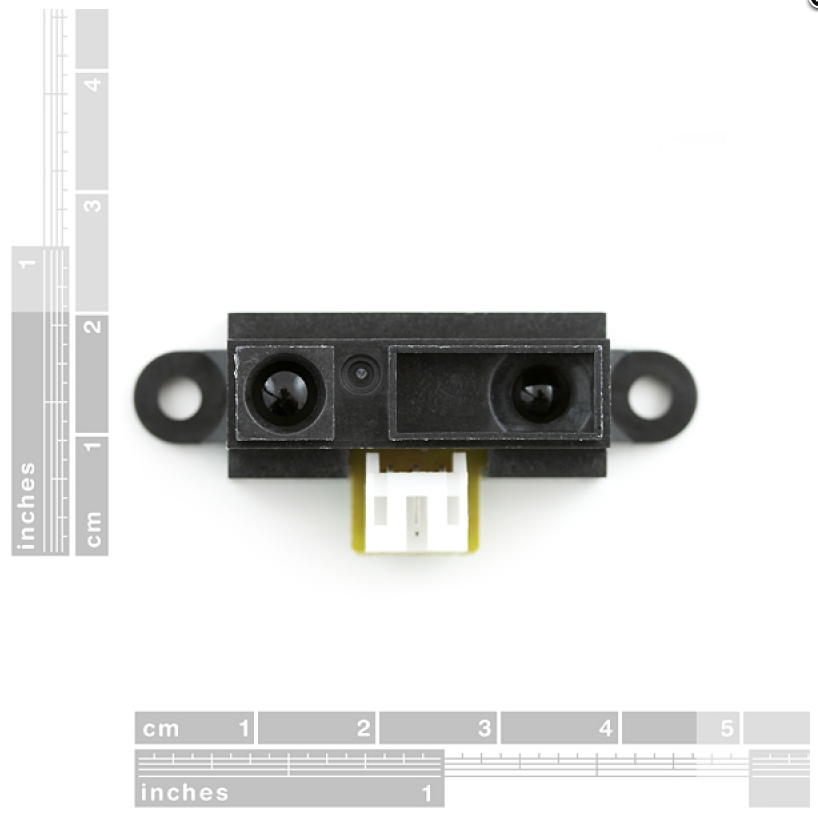
\includegraphics[page=1,width=0.35\textwidth]{img/sensor.png} 
\caption{Odometric Infrared Sensor GP2Y0A21YK}
\label{fig:sensor}
\end{figure}